\section{Generalising the model}

We have seen that HMM can be used to simulate rainfall similar to that given in the training data. While this is useful, it also has some limitations. For example, due to our discretised system with interger value groups, some groups have 0 probability. This is justified by the data but cannot be explained by nature. For example, for our selected attempt of 1 in month 0, given the system is in state 1, the probability of 1mm of rainfall is 0.0284927 however the probability of 2mm is 0. This may be true for the data but is not a reasonable assumption in nature. As such we must find a method to generalise the model. Generalising the observation matrix, such that the simulation not only reprsents the training data but is infact useful in simulating future rainfall patterns.

\section{Finding a function for Observation Matrix}

To generalise our model we require a function for each row of the observation matrix. We could test for polynomial fits but we will attempt to use our model as it has real life justifications. We propose our model, which was developed by adjusting Grando's Model.

\begin{prop}
    \label{model}
    Given the system is in state i, the amount of rainfall in mm is given by
    \begin{equation}
        \sum_{i=0}^N \sigma_i
    \end{equation}
    where $N \sim pois(\lambda)$ is the number of storm discs and $\sigma \sim exp(\tau)$ is the intensity of rain in each.
\end{prop}



\section{Parameter Estimation}


For each row of each observation matrix, according to \ref{model}, we have two unknown parameters. In other words, for our example, we have six unknown paramters for each month. Fortuantely we do not have to attempt to estimate all of these from the same data. We can use the distribution, given by each row, to generate a simulation and then attempt to fit our two parameters to this.


- For given min and max lambda and tau, simulate rainfall, calculate frequencies and find absolute difference ebtween this and freq in row given by matrix B.
- Analysis done in R
- Plot 3D graph of lambda, tau and residual, look for minimum
- Repeat, optimising min and max lam and tau each time 
- Look for hyperbola in tau-residual and lam-residual graphs and find minimum. 
- Record minimum values as parameter estimates

Model Generation
- Simply go through HMM and other model features using parameter estimates found in prev.


\subsection{Methodology}

The programs used for this are "pe" and "Analysis.R" both in the parameter estiation folder. The program "pe" follows the following steps:
\begin{enumerate}
    \item Input of the minimum and maximum value desired of $\lambda$ and $\tau$ as well as which row is being fit.
    \item Uniformly randomly selects values within the given ranges and generate a simulation of size 100000 for the given row.
    \item Create array contating freqency counts of each integer from simulation.
    \item Using observation matrix row as a distribution, find expected frequency for 100000 simulations by multiplying probability by number of iterations. Store results in array.
    \item Find difference between each element of frequency of simulation and freqency of expectation array. Sum absolute value of each and take this value as residual for given $\lambda$ and $\tau$. 
    \item Repeat steps 1000 times for given $\lambda$ and $\tau$. Record $\lambda$ and $\tau$ and residual in csv file. 
\end{enumerate}



\subsection{Results}
"pe" has been optimised to run over up to 24 threads. Due to this, when given the 24 threads,  the program finishes the above computation within 10-30 seconds.


"Analysis.R" is used to analyse the csv file. It plots three graphs; a 3D graph of $\lambda$ against $\tau$ against residual, $\lambda$ against residual and $\tau$ against residual. We use these three graphs to find an approximate area of $\lambda$ or $\tau$ where residual is lowest and then repeat "pe" for this new area. 

We will demonstrate the results for the first row of the observatino matrix for Month 0. The process followed for calculating all other parameter estimates has been the same. 

\begin{figure}
    \begin{subfigure}{.8\textwidth}
      \centering
      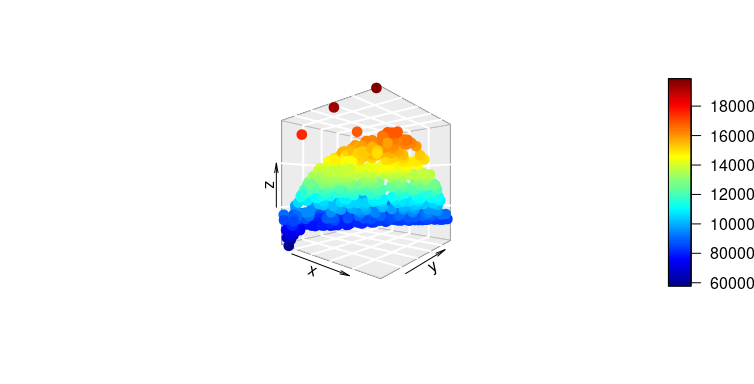
\includegraphics[width=\linewidth]{Parameter Estimation on Attempt _1/param_1/lam0-10tau0-10.png}
      \caption{}
      \label{pe1:1}
    \end{subfigure}

    \begin{subfigure}{.45\textwidth}
      \centering
      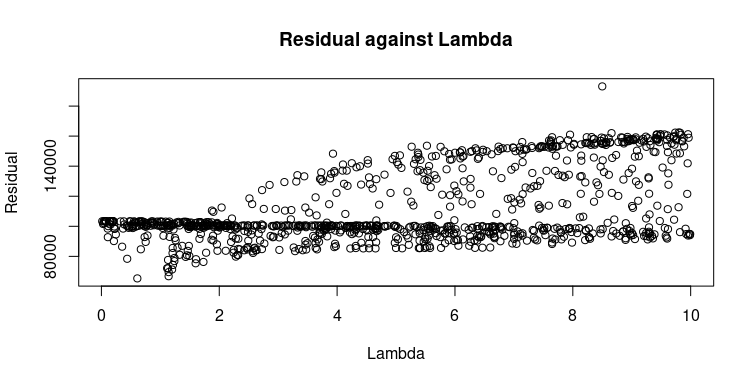
\includegraphics[width=\linewidth]{Parameter Estimation on Attempt _1/param_1/lam_1.png}
      \caption{}
      \label{pe1:2}
    \end{subfigure}
    \begin{subfigure}{.45\textwidth}
      \centering
      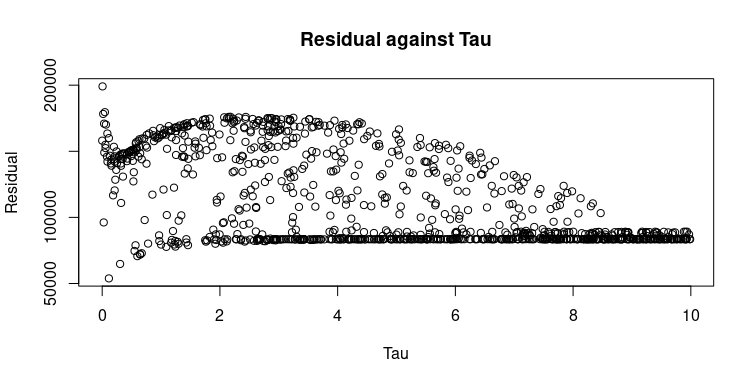
\includegraphics[width=\linewidth]{Parameter Estimation on Attempt _1/param_1/tau_1.png}
      \caption{}
      \label{pe1:3}
    \end{subfigure}
    \caption{}
    \label{pe1}
\end{figure}

\begin{figure}
    \begin{subfigure}{.8\textwidth}
      \centering
      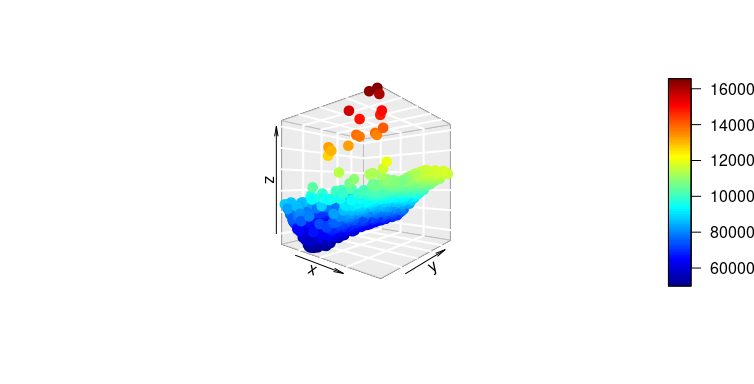
\includegraphics[width=\linewidth]{Parameter Estimation on Attempt _1/param_1/lam0-2tau0-0_5.png}
      \caption{}
      \label{pe2:1}
    \end{subfigure}

    \begin{subfigure}{.45\textwidth}
      \centering
      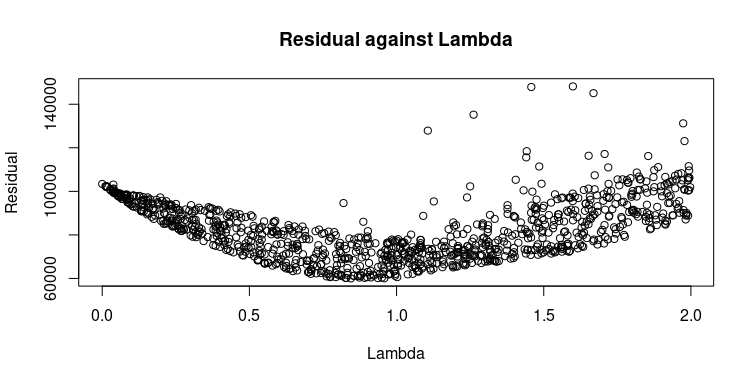
\includegraphics[width=\linewidth]{Parameter Estimation on Attempt _1/param_1/lam_2.png}
      \caption{}
      \label{pe2:2}
    \end{subfigure}
    \begin{subfigure}{.45\textwidth}
      \centering
      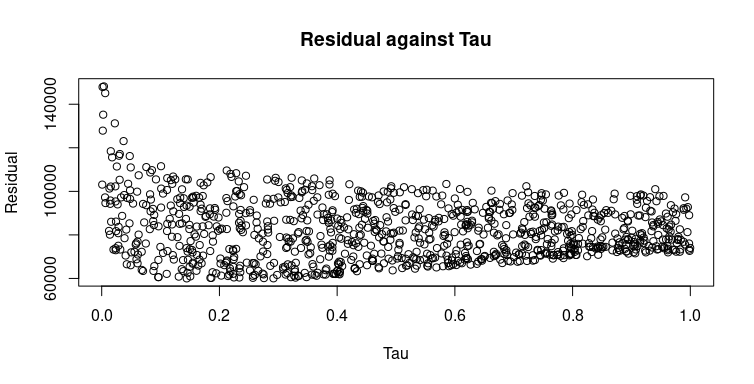
\includegraphics[width=\linewidth]{Parameter Estimation on Attempt _1/param_1/tau_2.png}
      \caption{}
      \label{pe2:3}
    \end{subfigure}
    \caption{}
    \label{pe2}
\end{figure}

\begin{figure}
    \begin{subfigure}{.8\textwidth}
      \centering
      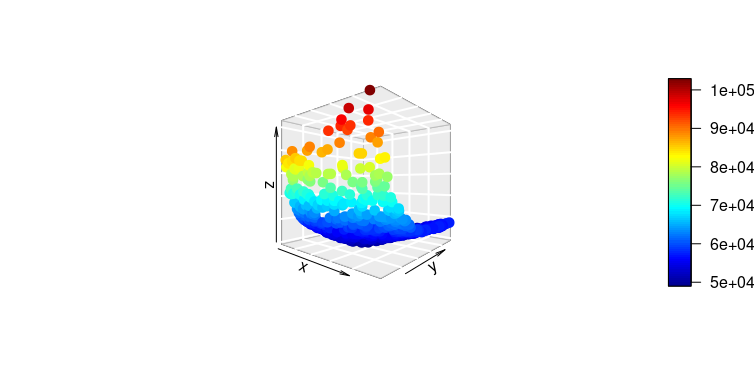
\includegraphics[width=\linewidth]{Parameter Estimation on Attempt _1/param_1/lam0_5-0_75tau0-0_1.png}
      \caption{}
      \label{pe3:1}
    \end{subfigure}

    \begin{subfigure}{.45\textwidth}
      \centering
      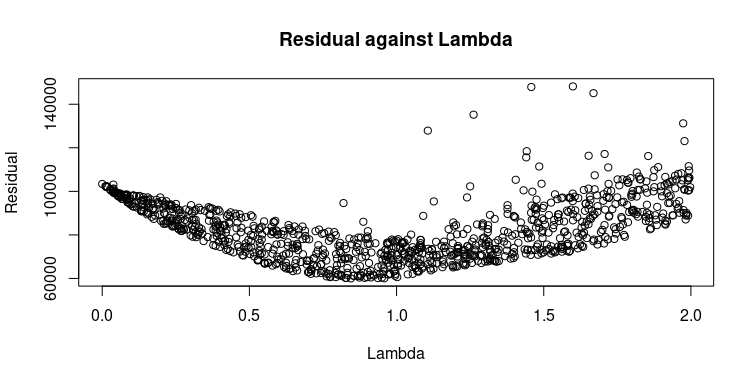
\includegraphics[width=\linewidth]{Parameter Estimation on Attempt _1/param_1/lam_3.png}
      \caption{}
      \label{pe3:2}
    \end{subfigure}
    \begin{subfigure}{.45\textwidth}
      \centering
      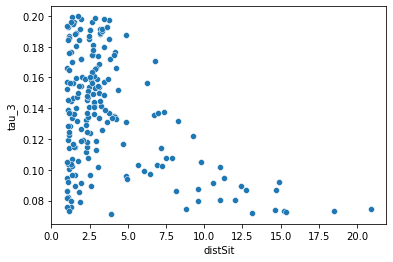
\includegraphics[width=\linewidth]{Parameter Estimation on Attempt _1/param_1/tau_3.png}
      \caption{}
      \label{pe3:3}
    \end{subfigure}
    \caption{}
    \label{pe3}
\end{figure}

We begin by running "pe" between 0-10 for both tau and lambda. Through initial testing with random ranges we found that both values tend to have their minimum residual points within these ranges. It is clear from Figure \ref{pe1} that $\lambda \in [0,2]$ and $\tau \in [0,0.5]$. Thus we repeat the program for this new range, the results can be seen in figure \ref{pe2}. This time we can see that $\lambda \in [0.5,0.75]$ and $\tau \in [0,0.1]$. We repeat the program one more time with these new ranges and retrieve Figure \ref{pe3}. We can now approximate that $\lambda \approx 0.625$ and $\tau \approx 0.05$. 

We repeat this process for every row of the observation matrix for every month. The results are as given:

\begin{center}
    \begin{tabular}{c c c c c c c}
        \label{petable}
        Month	&   Lambda 1	&   Lambda 2	&   Lambda 3	&   Tau 1 	&   Tau 2	&   Tau 3   \\
            0	&   0.625	    &   0.9	        &   0.775	    &   0.05	&   0.2	    &   0.06    \\
            1	&   0.265	    &   3.25	    &   1.95	    &   0.06	&   0.15	&   0.055   \\
            2	&   0.42	    &   3.3	        &   4	        &   0.09	&   0.11	&   0.1     \\
            3	&   2.5	        &   2.5	        &   0.35	    &   0.12	&   0.175	&   0.06    \\
            4	&   2.3	        &   3.25	    &   0.525	    &   0.09	&   0.16	&   0.075   \\
            5	&   4	        &   1.55	    &   0.3	        &   0.13	&   0.1	    &   0.06    \\
            6	&   2.25	    &   0.6	        &   0.55	    &   0.075	&   0.075	&   0.075   \\
            7	&   3.4	        &   0.24	    &   2.15	    &   0.2	    &   0.075	&   0.1     \\
            8	&   0.57	    &   0.52	    &   3.2	        &   0.04	&   0.06	&   0.12    \\
            9	&   5.5	        &   0.3	        &   2.6	        &   0.17	&   0.05	&   0.25    \\
            10	&   0.27	    &   9	        &   2.75	    &   0.05	&   0.64	&   0.075   \\
            11	&   4.15	    &   0.24	    &   2	        &   0.1	    &   0.075	&   0.11    

    \end{tabular}
\end{center}

We can see from table \ref{petable} that while the values of $\tau$ are often similar, lambda values vary drastically. Regardless, we are concerned with the performance of this model. In the next chapter we test this model as well as apply more rigourous tests on the hmm only model.